\documentclass{csbeamer}

\usepackage{dsfont}

% Add custom color definitions for consistency
\definecolor{robotblue}{HTML}{4285F4}
\definecolor{robotred}{HTML}{EA4335}
\definecolor{robotgreen}{HTML}{34A853}
\definecolor{robotyellow}{HTML}{FBBC05}
\definecolor{banditmain}{HTML}{6A4C93}
\definecolor{banditaccent}{HTML}{F72585}
\definecolor{banditlight}{HTML}{C77DFF}
\definecolor{banditsecondary}{HTML}{7209B7}

\university{St. Francis Xavier University}
\department{Department of Computer Science}
\course{CSCI-531 - Reinforcement Learning}
\courseshort{CSCI-531 - RL}
\term{Fall 2025}
\author{Dr. Jean-Alexis Delamer}

\title{Multi-Armed Bandit}

\begin{document}

\frame{\titlepage}

% Section: Introduction
\section{Introduction}

% Subsection: From Full RL to Bandits
\subsection{From Full RL to Bandits}

\begin{frame}
    \frametitle{From Full RL to Bandit Problems}

    \begin{block}<1->{Why Start with Bandits?}
        \begin{itemize}
            \item<1-> Multi-armed bandits are a \textcolor{banditmain}{\textbf{simplified version}} of full RL
            \item<2-> Focus on one key aspect: the \textcolor{banditaccent}{\textbf{exploration-exploitation trade-off}}
            \item<3-> Foundation for understanding more complex RL scenarios
        \end{itemize}
    \end{block}

    \begin{block}<4->{Relationship to Full RL}
        \begin{itemize}
            \item<4-> \textbf{Bandit}: Single state, multiple actions, immediate rewards
            \item<5-> \textbf{Full RL}: Multiple states, multiple actions, delayed rewards
            \item<6-> \textcolor{robotgreen}{\textbf{Key insight}}: Every state in full RL = separate bandit problem
        \end{itemize}
    \end{block}

    \only<7->{
        \begin{center}
            \textcolor{banditsecondary}{\textit{Understanding bandits $\rightarrow$ Foundation for all RL}}
        \end{center}
    }
\end{frame}

% Subsection: The k-Armed Bandit Problem
\subsection{The k-Armed Bandit Problem}

\begin{frame}
    \frametitle{What is the k-Armed Bandit Problem?}

    \begin{columns}
        \begin{column}{0.6\textwidth}
            \begin{block}<1->{The Setup}
                \begin{itemize}
                    \item<1-> Agent has $k$ different actions
                    \item<2-> After taking action $\rightarrow$ receive reward
                    \item<3-> Rewards from \textcolor{banditmain}{stationary probability distribution}
                    \item<4-> \textbf{Objective}: Maximize expected total reward
                \end{itemize}
            \end{block}
        \end{column}

        \begin{column}{0.4\textwidth}
            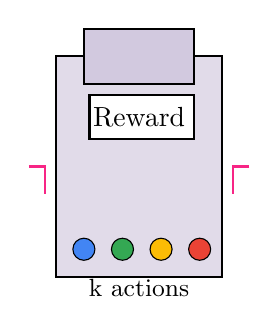
\begin{tikzpicture}[scale=0.7]
                % Slot machine representation
                % Machine body
                \draw<1->[thick, fill=banditmain!20] (0,0) rectangle (3,4);
                \draw<1->[thick, fill=banditmain!30] (0.5,3.5) rectangle (2.5,4.5);

                % Arms/levers
                \draw<2->[thick, banditaccent] (-0.5,2) -- (-0.2,2) -- (-0.2,1.5);
                \draw<2->[thick, banditaccent] (3.5,2) -- (3.2,2) -- (3.2,1.5);

                % Action buttons
                \draw<2->[fill=robotblue] (0.5,0.5) circle (0.2);
                \draw<2->[fill=robotgreen] (1.2,0.5) circle (0.2);
                \draw<2->[fill=robotyellow] (1.9,0.5) circle (0.2);
                \draw<2->[fill=robotred] (2.6,0.5) circle (0.2);

                % Display
                \draw<3->[thick, fill=white] (0.6,2.5) rectangle (2.5,3.3);
                \node<3-> at (1.5,2.9) {Reward};

                % Labels
                \node<2-> at (1.5,-0.2) {\small{k actions}};
            \end{tikzpicture}
        \end{column}
    \end{columns}
\end{frame}

\begin{frame}
    \frametitle{Mathematical Formulation}

    \begin{block}<1->{Key Variables}
        \begin{itemize}
            \item<1-> \textbf{Action at time $t$}: $A_t \in \{1, 2, \ldots, k\}$
            \item<2-> \textbf{Corresponding reward}: $R_t$
            \item<3-> \textbf{Reward distribution}: $R_t \sim P(r | A_t)$
        \end{itemize}
    \end{block}

    \begin{block}<4->{True vs Estimated Values}
        \textbf{True value of action $a$:}
        \begin{equation*}
            q_*(a) = \mathbb{E}[R_t | A_t = a]
        \end{equation*}

        \textbf{Estimated value at time $t$:}
        \begin{equation*}
            Q_t(a) \approx q_*(a)
        \end{equation*}
    \end{block}

    \only<5->{
        \begin{center}
            \textcolor{banditaccent}{\textbf{Challenge: We don't know $q_*(a)$ - must estimate from experience!}}
        \end{center}
    }
\end{frame}

\begin{frame}
    \frametitle{The Exploration-Exploitation Dilemma}

    \begin{columns}
        \begin{column}{0.6\textwidth}
            \begin{block}<1->{When you know $Q_t(a)$ for all actions:}
                \begin{itemize}
                    \item<2-> \textcolor{robotgreen}{\textbf{Exploitation}}: Choose $\arg\max_a Q_t(a)$
                        \begin{itemize}
                            \item<2-> Greedy action selection
                            \item<3-> Maximizes immediate reward
                            \item<4-> \textcolor{robotred}{But estimates might be wrong!}
                        \end{itemize}
                    \item<5-> \textcolor{robotblue}{\textbf{Exploration}}: Choose non-greedy actions
                        \begin{itemize}
                            \item<5-> Improves action-value estimates
                            \item<6-> Necessary for long-term success
                            \item<7-> \textcolor{robotred}{But sacrifices immediate reward}
                        \end{itemize}
                \end{itemize}
            \end{block}
        \end{column}

        \begin{column}{0.4\textwidth}
            \begin{tikzpicture}[scale=0.8]
                % Show exploitation vs exploration visually
                \only<2-4>{
                    % Exploitation
                    \draw[thick, fill=robotgreen!20] (0,2) rectangle (3,3);
                    \node at (1.5,2.5) {\textbf{Exploitation}};

                    % Best known action
                    \draw[fill=robotgreen] (0.5,1.5) circle (0.2);
                    \node at (0.5,1.2) {Best};

                    % Arrow pointing to best
                    \draw<3->[->, thick, robotgreen] (1.5,2) to[bend right] (0.7,1.7);

                    \node<4-> at (1.5,0.8) {\textcolor{robotred}{\textbf{Risk: Wrong estimate!}}};
                }

                \only<5-7>{
                    % Exploration
                    \draw[thick, fill=robotblue!20] (0,2) rectangle (3,3);
                    \node at (1.5,2.5) {\textbf{Exploration}};

                    % Multiple actions
                    \draw[fill=robotblue] (0.3,1.5) circle (0.15);
                    \draw[fill=robotblue] (0.9,1.5) circle (0.15);
                    \draw[fill=robotblue] (1.5,1.5) circle (0.15);
                    \draw[fill=robotblue] (2.1,1.5) circle (0.15);
                    \draw[fill=robotblue] (2.7,1.5) circle (0.15);

                    % Arrows to different actions
                    \draw<6->[->, thick, robotblue] (0.8,2) to[bend left] (0.5,1.7);
                    \draw<6->[->, thick, robotblue] (1.5,2) to (1.5,1.7);
                    \draw<6->[->, thick, robotblue] (2.2,2) to[bend right] (2.5,1.7);

                    \node<7-> at (1.5,0.8) {\textcolor{robotred}{\textbf{Cost: Lower immediate reward}}};
                }
            \end{tikzpicture}
        \end{column}
    \end{columns}

    \only<8->{
        \begin{center}
            \large{\textcolor{banditmain}{\textbf{The Challenge: Balance exploration and exploitation}}}
        \end{center}
    }
\end{frame}

% Section: Action-Value Methods
\section{Action-Value Methods}

\subsection{Estimating Action Values}

\begin{frame}
    \frametitle{Action-Value Methods}

    \begin{block}<1->{The Approach}
        \begin{enumerate}
            \item<1-> \textbf{Estimate} action values from experience
            \item<2-> \textbf{Use} these estimates to select actions
            \item<3-> \textbf{Update} estimates as we gain more experience
        \end{enumerate}
    \end{block}

    \begin{block}<4->{Why This Works}
        \begin{itemize}
            \item<4-> We observe rewards for each action we take
            \item<5-> More samples $\rightarrow$ better estimates
            \item<6-> Can balance exploration (trying new actions) vs exploitation (using best known action)
        \end{itemize}
    \end{block}

    \only<7->{
        \begin{center}
            \textcolor{banditmain}{\textbf{How do we estimate action values?}}
        \end{center}
    }
\end{frame}

\begin{frame}
    \frametitle{Sample Average Method}

    \begin{block}<1->{Natural Estimation Approach}
        One natural way to estimate expected reward:
        \begin{equation*}
            Q_t(a) = \frac{\text{sum of rewards when } a \text{ taken prior to } t}{\text{number of times } a \text{ taken prior to } t}
        \end{equation*}
    \end{block}

    \begin{block}<2->{Mathematical Formulation}
        More formally:
        \begin{equation*}
            Q_t(a) = \frac{\sum_{i=1}^{t-1} R_i \cdot \mathds{1}_{A_i=a}}{\sum_{i=1}^{t-1} \mathds{1}_{A_i=a}}
        \end{equation*}
        where $\mathds{1}_{A_i=a}$ is 1 if action $a$ was taken at time $i$, 0 otherwise.
    \end{block}

    \only<3->{
        \begin{center}
            \textcolor{robotgreen}{\textbf{Law of Large Numbers}: As $n \rightarrow \infty$, $Q_t(a) \rightarrow q_*(a)$}
        \end{center}
    }
\end{frame}

\begin{frame}
    \frametitle{Example: Estimating Action Values}

    \begin{center}
        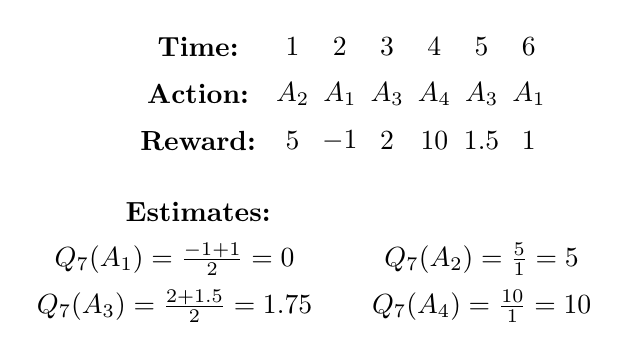
\begin{tikzpicture}[scale=0.6]
            % Timeline of actions and rewards
            \node at (-1,4) {\textbf{Time:}};
            \node at (-1,3) {\textbf{Action:}};
            \node at (-1,2) {\textbf{Reward:}};

            % Time steps
            \foreach \t in {1,2,3,4,5,6} {
                \node at (\t,4) {$\t$};
            }

            % Actions taken (example sequence)
            \node at (1,3) {$A_2$};
            \node at (2,3) {$A_1$};
            \node at (3,3) {$A_3$};
            \node at (4,3) {$A_4$};
            \node at (5,3) {$A_3$};
            \node at (6,3) {$A_1$};

            % Rewards received
            \node at (1,2) {$5$};
            \node at (2,2) {$-1$};
            \node at (3,2) {$2$};
            \node at (4,2) {$10$};
            \node at (5,2) {$1.5$};
            \node at (6,2) {$1$};

            % Calculations
            \node at (-1,0.5) {\textbf{Estimates:}};
            \node at (-1.5,-0.5) {$Q_7(A_1) = \frac{-1+1}{2} = 0$};
            \node at (5,-0.5) {$Q_7(A_2) = \frac{5}{1} = 5$};
            \node at (-1.5,-1.5) {$Q_7(A_3) = \frac{2+1.5}{2} = 1.75$};
            \node at (5,-1.5) {$Q_7(A_4) = \frac{10}{1} = 10$};
        \end{tikzpicture}
    \end{center}

    \begin{center}
        \textcolor{banditmain}{\textbf{Best action so far: }} $A_4$ with $Q_7(A_4) = 10$
    \end{center}
\end{frame}

\subsection{Action Selection Strategies}

\begin{frame}
    \frametitle{$\epsilon$-Greedy Action Selection}

    \begin{block}<1->{The Strategy}
        Balance exploration and exploitation with a simple rule:
        \begin{itemize}
            \item<2-> With probability $(1-\epsilon)$: Choose \textcolor{robotgreen}{\textbf{greedy action}}
                \begin{equation*}
                    A_t = \arg\max_a Q_t(a)
                \end{equation*}
            \item<3-> With probability $\epsilon$: Choose \textcolor{robotblue}{\textbf{random action}}
                \begin{equation*}
                    A_t = \text{uniform random from all actions}
                \end{equation*}
        \end{itemize}
    \end{block}

    \only<4->{
        \begin{center}
            \textcolor{banditmain}{\textbf{Simple but effective approach to exploration-exploitation}}
        \end{center}
    }
\end{frame}

\begin{frame}
    \frametitle{$\epsilon$-Greedy Parameter Analysis}

    \begin{block}<1->{Parameter $\epsilon$}
        \begin{itemize}
            \item<1-> $\epsilon = 0$: Pure exploitation (greedy)
            \item<2-> $\epsilon = 1$: Pure exploration (random)
            \item<3-> $\epsilon \in (0,1)$: Balanced approach
        \end{itemize}
    \end{block}

    \begin{block}<4->{Properties}
        \begin{itemize}
            \item<4-> \textcolor{robotgreen}{\textbf{Guarantees convergence}} to optimal action
            \item<5-> \textcolor{robotred}{\textbf{But}} doesn't guarantee optimal performance
            \item<6-> Simple to implement and understand
        \end{itemize}
    \end{block}

    \only<7->{
        \begin{center}
            \textcolor{banditaccent}{\textbf{Trade-off: Higher $\epsilon$ = more exploration, lower immediate reward}}
        \end{center}
    }
\end{frame}

\begin{frame}
    \frametitle{$\epsilon$-Greedy Example}

    \begin{columns}
        \begin{column}{0.6\textwidth}
            \textbf{Current estimates:}
            \begin{align*}
                Q_t(A_1) &= 0 \\
                Q_t(A_2) &= 5 \\
                Q_t(A_3) &= 1.75 \\
                Q_t(A_4) &= 10 \quad \textcolor{robotgreen}{\leftarrow \text{Best}}
            \end{align*}

            \textbf{With $\epsilon = 0.1$:}
            \begin{itemize}
                \item Probability of choosing $A_4$: $0.9 + 0.1 \times 0.25 = 0.925$
                \item Probability of choosing any other action: $0.1 \times 0.25 = 0.025$
            \end{itemize}
        \end{column}

        \begin{column}{0.4\textwidth}
            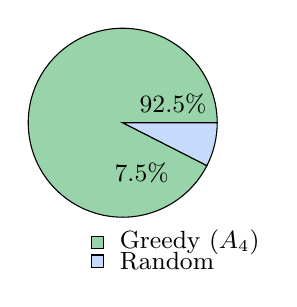
\begin{tikzpicture}[scale=0.8]
                % Pie chart showing probabilities
                \draw[fill=robotgreen!50] (0,0) -- (0:1.5) arc (0:333:1.5) -- cycle;
                \draw[fill=robotblue!30] (0,0) -- (333:1.5) arc (333:360:1.5) -- cycle;

                % Labels
                \node at (0.8,0.3) {\small{92.5\%}};
                \node at (0.3,-0.8) {\small{7.5\%}};

                % Legend
                \draw[fill=robotgreen!50] (-0.5,-2) rectangle (-0.3,-1.8);
                \node[right] at (-0.2,-1.9) {\small{Greedy ($A_4$)}};

                \draw[fill=robotblue!30] (-0.5,-2.3) rectangle (-0.3,-2.1);
                \node[right] at (-0.2,-2.2) {\small{Random}};
            \end{tikzpicture}
        \end{column}
    \end{columns}
\end{frame}

% Section: Incremental Implementation
\section{Incremental Implementation}

\subsection{Efficient Computation}

\begin{frame}
    \frametitle{The Computational Challenge}

    \begin{block}<1->{Naive Implementation}
        Store all rewards and recompute average each time:
        \begin{equation*}
            Q_n = \frac{R_1 + R_2 + \cdots + R_{n-1}}{n-1}
        \end{equation*}

        \textcolor{robotred}{\textbf{Problems:}}
        \begin{itemize}
            \item<2-> Memory grows linearly with time
            \item<3-> Computation time increases with each update
        \end{itemize}
    \end{block}

    \only<4->{
        \begin{center}
            \textcolor{banditaccent}{\textbf{Better approach needed.}}
        \end{center}
    }
\end{frame}

\begin{frame}
    \frametitle{Incremental Update Rule}

    \begin{block}<1->{Mathematical Derivation}
        Starting with the sample average:
        \begin{align*}
            Q_{n+1} &= \frac{1}{n}\sum_{i=1}^n R_i
            \onslide<2->{= \frac{1}{n}\left(R_n + \sum_{i=1}^{n-1} R_i\right) \\}
            \onslide<3->{&= \frac{1}{n}\left(R_n + (n-1) \frac{1}{n-1}\sum_{i=1}^{n-1} R_i\right) \\}
            \onslide<4->{&= \frac{1}{n}\left(R_n + (n-1) Q_n\right)}
            \onslide<5->{= \frac{1}{n} R_n + \frac{n-1}{n} Q_n \\}
            \onslide<6->{&= Q_n + \frac{1}{n}\left[R_n - Q_n\right]}
        \end{align*}
    \end{block}

    \only<7->{
        \begin{center}
            \large{$Q_{n+1} = Q_n + \frac{1}{n}[R_n - Q_n]$}
        \end{center}
    }
\end{frame}

\begin{frame}
    \frametitle{The General Update Form}

    \begin{block}{Key RL Update Pattern}
        \begin{equation*}
            \text{NewEstimate} \leftarrow \text{OldEstimate} \quad + \text{StepSize} \times [\text{Target} - \text{OldEstimate}]
        \end{equation*}
    \end{block}

    \begin{block}<2->{Components}
        \begin{itemize}
            \item<2-> \textcolor{robotgreen}{\textbf{Target}}: $R_n$ (the observed reward)
            \item<3-> \textcolor{robotblue}{\textbf{Prediction Error}}: $[R_n - Q_n]$
            \item<4-> \textcolor{banditmain}{\textbf{Step Size}}: $\frac{1}{n}$ (how much to adjust)
        \end{itemize}
    \end{block}

    \only<5->{
        \begin{center}
            \textcolor{banditaccent}{\textit{This pattern appears throughout all of reinforcement learning!}}
        \end{center}
    }
\end{frame}

\begin{frame}[fragile]
    \frametitle{Complete k-Armed Bandit Algorithm}

    \begin{algorithm}[H]
    \caption{$\epsilon$-Greedy k-Armed Bandit}
    \begin{algorithmic}[1]
    \State \textbf{Initialize:}
    \For{$a = 1$ to $k$}
        \State $Q(a) \leftarrow 0$
        \State $N(a) \leftarrow 0$
    \EndFor
    \State \textbf{Loop forever:}
    \State $A \leftarrow \begin{cases} \arg\max_a Q(a) \quad \text{with probability } 1-\epsilon \\ \text{random action} \end{cases}$
    \State $R \leftarrow$ bandit($A$)
    \State $N(A) \leftarrow N(A) + 1$
    \State $Q(A) \leftarrow Q(A) + \frac{1}{N(A)}[R - Q(A)]$
    \end{algorithmic}
    \end{algorithm}
\end{frame}

% Section: Advanced Methods
\section{Advanced Methods}

\subsection{Constant Step-Size}

\begin{frame}
    \frametitle{Beyond Sample Averages: Constant Step-Size}

    \begin{block}<1->{Limitation of Sample Average}
        Sample average method: $Q_{n+1} = Q_n + \frac{1}{n}[R_n - Q_n]$
        \begin{itemize}
            \item<2-> Gives \textcolor{robotred}{\textbf{equal weight}} to all past rewards
            \item<3-> Step size $\frac{1}{n}$ decreases over time
            \item<4-> \textcolor{robotred}{\textbf{Problem}}: Old rewards have too much influence
        \end{itemize}
    \end{block}

    \begin{block}<5->{Constant Step-Size Alternative}
        Replace $\frac{1}{n}$ with constant $\alpha \in (0,1]$:
        \begin{equation*}
            Q_{n+1} = Q_n + \alpha[R_n - Q_n]
        \end{equation*}

        \textcolor{robotgreen}{\textbf{Benefits:}}
        \begin{itemize}
            \item<6-> More weight to recent rewards
            \item<7-> Called \textbf{weighted average}
        \end{itemize}
    \end{block}
\end{frame}

\begin{frame}
    \frametitle{Weighted Average Derivation}

    \begin{block}<1->{Expanding the Constant Step-Size Update}
        \begin{align*}
            Q_{n+1} &= Q_n + \alpha[R_n - Q_n] \\
            \onslide<2->{&= (1-\alpha)Q_n + \alpha R_n \\}
            \onslide<3->{&= (1-\alpha)[(1-\alpha)Q_{n-1} + \alpha R_{n-1}] + \alpha R_n \\}
            \onslide<4->{&= (1-\alpha)^2 Q_{n-1} + \alpha(1-\alpha)R_{n-1} + \alpha R_n \\}
            \onslide<5->{&= \cdots \\}
            \onslide<6->{&= (1-\alpha)^n Q_1 + \sum_{i=1}^n \alpha(1-\alpha)^{n-i} R_i}
        \end{align*}
    \end{block}

\end{frame}

\begin{frame}
\frametitle{Weighted Average Derivation}

\begin{block}<1->{Expanding the Constant Step-Size Update}
    \begin{align*}
        Q_{n+1} = (1-\alpha)^n Q_1 + \sum_{i=1}^n \alpha(1-\alpha)^{n-i} R_i
    \end{align*}
\end{block}

\only<2->{
    \textcolor{banditmain}{\textbf{Weight of reward $R_i$}}: $\alpha(1-\alpha)^{n-i}$

    \begin{itemize}
        \item Recent rewards have weight close to $\alpha$
        \item Weights decay exponentially into the past
        \item Sum of all weights = 1 (true weighted average)
    \end{itemize}
}
\end{frame}

\subsection{Upper Confidence Bound}

\begin{frame}
    \frametitle{Upper Confidence Bound (UCB) Action Selection}

    \begin{block}<1->{Limitation of $\epsilon$-Greedy}
        \begin{itemize}
            \item<1-> Random exploration among \textbf{all} non-greedy actions
            \item<2-> No preference for actions with high uncertainty
            \item<3-> Doesn't consider \textcolor{robotred}{\textbf{how uncertain}} our estimates are
        \end{itemize}
    \end{block}

    \begin{block}<4->{UCB Idea}
        \textcolor{banditmain}{\textbf{Explore based on uncertainty!}}
        \begin{itemize}
            \item<5-> High uncertainty $\rightarrow$ more exploration
            \item<6-> Low uncertainty $\rightarrow$ less exploration
            \item<7-> Select action with highest \textbf{upper confidence bound}
        \end{itemize}
    \end{block}
\end{frame}

\begin{frame}
    \frametitle{Understanding the UCB Formula}

    \begin{equation*}
        A_t = \arg\max_a \left[ \underbrace{Q_t(a)}_{\text{Exploitation}} + \underbrace{c\sqrt{\frac{\ln t}{N_t(a)}}}_{\text{Exploration Bonus}} \right]
    \end{equation*}

    where $c > 0$ controls the degree of exploration

    \begin{block}<1->{Exploration Bonus Analysis}
        \begin{itemize}
            \item<2-> \textcolor{robotgreen}{\textbf{$N_t(a)$ increases}}: Uncertainty decreases $\rightarrow$ bonus decreases
            \item<3-> \textcolor{robotblue}{\textbf{$t$ increases}}: More total trials $\rightarrow$ should explore more
            \item<4-> \textcolor{banditmain}{\textbf{$c$ parameter}}: Controls exploration vs exploitation trade-off
        \end{itemize}
    \end{block}
\end{frame}


\begin{frame}
    \frametitle{Understanding the UCB Formula}

    \begin{equation*}
        A_t = \arg\max_a \left[ \underbrace{Q_t(a)}_{\text{Exploitation}} + \underbrace{c\sqrt{\frac{\ln t}{N_t(a)}}}_{\text{Exploration Bonus}} \right]
    \end{equation*}

    \begin{block}<1->{Intuition}
        \begin{itemize}
            \item<2-> Actions with few trials get high bonus (high uncertainty)
            \item<3-> Actions with many trials get low bonus (low uncertainty)
            \item<4-> Automatically balances exploration and exploitation
        \end{itemize}
    \end{block}

    \only<5->{
        \begin{center}
            \textcolor{banditaccent}{\textbf{No parameters to tune over time - UCB adapts automatically!}}
        \end{center}
    }
\end{frame}


\begin{frame}
    \frametitle{UCB Example}
    \vspace{-0.5em}

    \textbf{Current state after 8 time steps:}
    \vspace{-0.3em}
    \begin{align*}
        Q_8(A_1) &= 0, \quad N_8(A_1) = 2 \quad Q_8(A_2) = 5, \quad N_8(A_2) = 1 \\
        Q_8(A_3) &= 1.75, \quad N_8(A_3) = 3 \quad Q_8(A_4) = 10, \quad N_8(A_4) = 2
    \end{align*}
    \vspace{-0.5em}

    \textbf{UCB values with $c = 2$:}
    \vspace{-0.3em}
    {\small
    \begin{align*}
        UCB_8(A_1) &= 0 + 2\sqrt{\frac{\ln 8}{2}} = 0 + 2\sqrt{1.04} = 2.04 \\
        UCB_8(A_2) &= 5 + 2\sqrt{\frac{\ln 8}{1}} = 5 + 2\sqrt{2.08} = 7.88 \\
        UCB_8(A_3) &= 1.75 + 2\sqrt{\frac{\ln 8}{3}} = 1.75 + 2\sqrt{0.69} = 3.42 \\
        UCB_8(A_4) &= 10 + 2\sqrt{\frac{\ln 8}{2}} = 10 + 2\sqrt{1.04} = 12.04
    \end{align*}
    }
\end{frame}

\subsection{Gradient Bandit}

\begin{frame}
    \frametitle{Gradient Bandit Algorithms}

    \begin{block}<1->{Different Approach}
        Instead of estimating action values, learn \textcolor{banditmain}{\textbf{action preferences}}:
        \begin{itemize}
            \item<2-> Maintain preference $H_t(a)$ for each action $a$
            \item<3-> Higher preference $\rightarrow$ action selected more often
            \item<4-> Use preferences in \textbf{softmax distribution}
        \end{itemize}
    \end{block}

    \begin{block}<5->{Softmax Action Selection}
        \begin{equation*}
            \pi_t(a) = P(A_t = a) = \frac{e^{H_t(a)}}{\sum_{b=1}^k e^{H_t(b)}}
        \end{equation*}
        where $\pi_t(a)$ is the probability of selecting action $a$ at time $t$.
    \end{block}
\end{frame}

\begin{frame}
    \frametitle{Gradient Bandit Algorithms}

    \begin{block}<1->{Softmax Action Selection}
        \begin{equation*}
            \pi_t(a) = P(A_t = a) = \frac{e^{H_t(a)}}{\sum_{b=1}^k e^{H_t(b)}}
        \end{equation*}
        where $\pi_t(a)$ is the probability of selecting action $a$ at time $t$.
    \end{block}

    \begin{block}<2->{Initial Conditions}
        \begin{itemize}
            \item<3-> Start with $H_1(a) = 0$ for all actions
            \item<4-> Initially: $\pi_1(a) = \frac{1}{k}$ (uniform distribution)
        \end{itemize}
    \end{block}
\end{frame}


\begin{frame}
    \frametitle{Gradient Bandit: Action Preferences}

    \begin{block}<1->{Key Insight}
        \begin{itemize}
            \item<1-> No need to estimate action values $q_*(a)$
            \item<2-> Instead, learn relative preferences between actions
            \item<3-> Preferences determine selection probabilities
        \end{itemize}
    \end{block}

    \begin{block}<4->{Preference Properties}
        \begin{itemize}
            \item<4-> Only \textbf{relative} differences matter
            \item<5-> Adding constant to all preferences: no effect on probabilities
            \item<6-> If $H_t(a) > H_t(b)$, then $\pi_t(a) > \pi_t(b)$
        \end{itemize}
    \end{block}
\end{frame}

\begin{frame}
    \frametitle{Gradient Bandit Update Rules}

    \begin{block}<1->{Stochastic Gradient Ascent Updates}
        \textbf{For the selected action:}
        \begin{equation*}
            H_{t+1}(A_t) = H_t(A_t) + \alpha(R_t - \bar{R}_t)(1 - \pi_t(A_t))
        \end{equation*}

        \textbf{For all other actions $a \neq A_t$:}
        \begin{equation*}
            H_{t+1}(a) = H_t(a) - \alpha(R_t - \bar{R}_t)\pi_t(a)
        \end{equation*}

        where $\bar{R}_t$ is the average of all rewards up to time $t$ (baseline).
    \end{block}

    \begin{block}<2->{Intuition}
        \begin{itemize}
            \item<3-> \textcolor{robotgreen}{\textbf{$R_t > \bar{R}_t$}}: Increase preference for $A_t$, decrease for others
            \item<4-> \textcolor{robotred}{\textbf{$R_t < \bar{R}_t$}}: Decrease preference for $A_t$, increase for others
            \item<5-> Baseline $\bar{R}_t$ provides context - what's "good" vs "bad"
        \end{itemize}
    \end{block}
\end{frame}

\subsection{Thompson Sampling}

\begin{frame}
    \frametitle{Thompson Sampling: Bayesian Approach}

    \begin{block}<1->{The Bayesian Philosophy}
        \begin{itemize}
            \item<1-> Maintain \textcolor{banditmain}{\textbf{belief distributions}} over true action values
            \item<2-> Use \textcolor{robotgreen}{\textbf{uncertainty}} to guide exploration naturally
            \item<3-> No exploration parameters to tune!
        \end{itemize}
    \end{block}

    \begin{block}<4->{Thompson Sampling Algorithm}
        At each time step:
        \begin{enumerate}
            \item<5-> \textbf{Sample} $\theta_a$ from belief distribution for each action $a$
            \item<6-> \textbf{Select} action $A_t = \arg\max_a \theta_a$
            \item<7-> \textbf{Observe} reward $R_t$
            \item<8-> \textbf{Update} belief distribution for $A_t$ using Bayesian inference
        \end{enumerate}
    \end{block}
\end{frame}


\begin{frame}
    \frametitle{Thompson Sampling: Bayesian Approach}

    \begin{block}<1->{Thompson Sampling Algorithm}
        At each time step:
        \begin{enumerate}
            \item<1-> \textbf{Sample} $\theta_a$ from belief distribution for each action $a$
            \item<1-> \textbf{Select} action $A_t = \arg\max_a \theta_a$
            \item<1-> \textbf{Observe} reward $R_t$
            \item<1-> \textbf{Update} belief distribution for $A_t$ using Bayesian inference
        \end{enumerate}
    \end{block}

    \begin{block}<2->{Why It Works}
        \begin{itemize}
            \item<3-> \textcolor{robotgreen}{\textbf{Probability matching}}: Prob(select action) = Prob(action is optimal)
            \item<4-> \textcolor{robotblue}{\textbf{Natural exploration}}: High uncertainty $\rightarrow$ more sampling variation
            \item<5-> \textcolor{banditmain}{\textbf{Theoretically optimal}} for many reward distributions
        \end{itemize}
    \end{block}
\end{frame}

% Section: Algorithm Comparison
\section{Algorithm Comparison}

\subsection{Performance Comparison}

\begin{frame}
    \frametitle{Bandit Algorithm Comparison}

    \begin{center}
    \small
    \begin{tabular}{|l|l|l|l|l|}
    \hline
    \textbf{Algorithm} & \textbf{Exploration} & \textbf{Parameters} & \textbf{Cost} & \textbf{Best Use} \\
    \hline
    $\epsilon$-greedy & Random & $\epsilon$ & Very Low & Simple baseline \\
    \hline
    UCB & Confidence & $c$ & Low & Principled exploration \\
    \hline
    Gradient & Preference & $\alpha$, baseline & Medium & Varying scales \\
    \hline
    Thompson & Bayesian & Prior params & Medium & Optimal exploration \\
    \hline
    \end{tabular}
    \end{center}

    \begin{block}<2->{When to Use Which?}
        \begin{itemize}
            \item<2-> \textcolor{robotgreen}{\textbf{$\epsilon$-greedy}}: Need interpretable, simple baseline
            \item<3-> \textcolor{robotblue}{\textbf{UCB}}: Want theoretical guarantees without parameter tuning
            \item<4-> \textcolor{banditmain}{\textbf{Gradient}}: Action values have very different scales
            \item<5-> \textcolor{banditaccent}{\textbf{Thompson}}: Want near-optimal exploration
        \end{itemize}
    \end{block}
\end{frame}

\subsection{Theoretical Guarantees}

\begin{frame}
    \frametitle{Theoretical Performance Guarantees}

    \begin{block}<1->{Regret Analysis}
        \textbf{Regret} = Total reward loss compared to always choosing optimal action
        \begin{equation*}
            \text{Regret}_T = T \cdot r^* - \sum_{t=1}^T R_t
        \end{equation*}
        where $r^* = \max_a q_*(a)$ is the optimal expected reward.
    \end{block}
\end{frame}

\begin{frame}
    \frametitle{Theoretical Performance Guarantees}

    \begin{block}{Algorithm Regret Bounds}
        \begin{center}
        \begin{tabular}{|l|l|}
        \hline
        \textbf{Algorithm} & \textbf{Regret Bound} \\
        \hline
        Random & $O(T)$ \\
        $\epsilon$-greedy (fixed $\epsilon$) & $O(T)$ \\
        $\epsilon$-greedy (decreasing $\epsilon$) & $O(\sqrt{T \ln T})$ \\
        UCB & $O(\sqrt{k T \ln T})$ \\
        Thompson Sampling & $O(\sqrt{kT})$ \\
        \hline
        \end{tabular}
        \end{center}
    \end{block}

    \only<2->{
        \textcolor{robotgreen}{\textbf{Key insight}}: Sublinear regret bounds ($O(T)$) mean the algorithm eventually finds the optimal action!
    }
\end{frame}

% Section: From Bandits to Full RL
\section{From Bandits to Full RL}

\subsection{Limitations and Extensions}

\begin{frame}
    \frametitle{From Bandits to Full Reinforcement Learning}

    \begin{block}<1->{What Bandits Taught Us}
        \begin{itemize}
            \item<1-> \textcolor{robotgreen}{\textbf{Exploration vs Exploitation}} trade-off
            \item<2-> \textcolor{robotblue}{\textbf{Value estimation}} from experience
            \item<3-> \textcolor{banditmain}{\textbf{Action selection}} strategies
            \item<4-> \textcolor{banditaccent}{\textbf{Learning from rewards}}
        \end{itemize}
    \end{block}

    \begin{block}<5->{Limitations of Bandits}
        \begin{itemize}
            \item<5-> \textcolor{robotred}{\textbf{Single state}}: All decisions in same context
            \item<6-> \textcolor{robotred}{\textbf{Immediate rewards}}: No delayed consequences
            \item<7-> \textcolor{robotred}{\textbf{Independent actions}}: Choices don't affect future situations
            \item<8-> \textcolor{robotred}{\textbf{Stationary environment}}: World doesn't change
        \end{itemize}
    \end{block}
\end{frame}

\begin{frame}
    \frametitle{The Jump to Full Reinforcement Learning}

    \begin{columns}
        \begin{column}{0.5\textwidth}
            \begin{block}<1->{Full RL Removes Limitations}
                \begin{itemize}
                    \item<1-> \textcolor{robotgreen}{\textbf{Multiple States}}: Different situations
                    \item<2-> \textcolor{robotblue}{\textbf{Sequential Decisions}}: Actions affect future states
                    \item<3-> \textcolor{banditmain}{\textbf{Delayed Rewards}}: Long-term consequences
                    \item<4-> \textcolor{banditaccent}{\textbf{Dynamic Environment}}: World changes with actions
                \end{itemize}
            \end{block}
        \end{column}

        \begin{column}{0.5\textwidth}
            \begin{tikzpicture}[scale=0.8]
                % State transition diagram
                \only<1->{
                    % States
                    \draw[fill=robotblue!20] (0,2) circle (0.4);
                    \draw[fill=robotgreen!20] (2,2) circle (0.4);
                    \draw[fill=robotyellow!20] (1,0) circle (0.4);

                    \node at (0,2) {$s_1$};
                    \node at (2,2) {$s_2$};
                    \node at (1,0) {$s_3$};
                }

                \only<2->{
                    % Transitions
                    \draw[->, thick] (0.4,2) to[bend left] (1.6,2);
                    \draw[->, thick] (1.6,2) to[bend left] (0.4,2);
                    \draw[->, thick] (0.3,1.6) to (0.7,0.4);
                    \draw[->, thick] (1.7,1.6) to (1.3,0.4);
                    \draw[->, thick] (1,0.4) to[bend right] (0.3,1.6);
                }

                \only<3->{
                    % Rewards
                    \node at (1,2.5) {\textcolor{robotred}{$R$}};
                    \node at (-0.8,1) {\textcolor{robotred}{$R$}};
                    \node at (2.8,1) {\textcolor{robotred}{$R$}};
                }
            \end{tikzpicture}
        \end{column}
    \end{columns}

    \begin{block}<5->{Mathematical Connection}
        \begin{itemize}
            \item<5-> \textbf{Bandit}: $Q(a)$ - value of action $a$
            \item<6-> \textbf{Full RL}: $Q(s,a)$ - value of action $a$ in state $s$
        \end{itemize}
    \end{block}

    \only<7->{
        \begin{center}
            \large{\textcolor{banditmain}{\textbf{Every state in RL = separate bandit problem!}}}
        \end{center}
    }
\end{frame}

\begin{frame}
    \frametitle{Summary}

    \begin{block}{Next: Markov Decision Processes}
        \begin{itemize}
            \item States, actions, transitions, and rewards
            \item Policies and value functions
            \item Bellman equations
            \item Dynamic programming solutions
        \end{itemize}
    \end{block}

    \begin{center}
        \large{\textcolor{banditmain}{\textbf{The exploration-exploitation foundation is set!}}}
    \end{center}
\end{frame}

\end{document}
